% !TEX TS-program = xelatex
% !TEX encoding = UTF-8 Unicode

% Tennessee Technological University
% ME4140 - Fall 2016 - Fall 2017 - Fall 2020 
% Tristan Hill - September 10, 2020
% Module 4 - Catkin Workspace

\documentclass[fleqn]{beamer} % for presentation (has nav buttons at bottom)

\usepackage{/home/thill/Documents/lectures/ros_lectures/ros_module}

\newcommand{\MNUM}{4\hspace{2mm}} % Module number
\newcommand{\TNUM}{---\hspace{2mm}} % Topic number - single topic for now
\newcommand{\moduletitle}{Catkin Workspace} % Titles and Stuff
%\newcommand{\topictitle}{---} 

\newcommand{\sectiontitleI}{Software Packages - Review} % More Titles and Stuff
\newcommand{\sectiontitleII}{Directory Structure - Linux and ROS}
\newcommand{\sectiontitleIII}{Catkin Workspace - Working Directory}
\newcommand{\sectiontitleIV}{Tutorial 4 - Create a Package}

\author{ME4140 - ROS Workshop}
\title{\GD Module \MNUM - \moduletitle}
\date{Mechanical Engineering\vspc Tennessee Technological University}

\begin{document}

\lstset{language=MATLAB,basicstyle=\ttfamily\small,showstringspaces=false}

\frame{\titlepage \center\begin{framed}\Large \textbf{Module \MNUM - \moduletitle}\end{framed} \vspace{5mm}}

% Section 0 - Outline
\frame{
	
	\large \textbf{Module \MNUM - \moduletitle} \vspace{3mm}\\
	
	\begin{itemize}
	
		\item \hyperlink{sectionI}{\sectiontitleI}    \vspc % Section I
		\item \hyperlink{sectionII}{\sectiontitleII} 	\vspc % Section II
		\item \hyperlink{sectionIII}{\sectiontitleIII} 	\vspc %Section III
		\item \hyperlink{sectionIV}{\sectiontitleIV} \vspc %Section IV	
	
	\end{itemize}

}

\section{\sectiontitleI}

	% Section I - Frame I
	\begin{frame}[label=sectionI] \small
		\frametitle{\sectiontitleI}
		
		{\large In general, software is organized in \href{http://wiki.ros.org/Packages}{packages}}

                \begin{itemize}
					\item Definition: A suite of programs that function as a single entity to accomplish a task, or group of related tasks.                           
                                                       
                
                    \item {\it Software in ROS is organized in packages. A package might contain ROS nodes, a ROS-independent library, a dataset, configuration files, a third-party piece of software, or anything else that logically constitutes a useful module.}** 
                    \item a collection of related nodes, each node belongs to a package
                     \item many pre-built packages with ros installation: {\fontfamily{qcr}\selectfont  {\bf -desktop-full}}
                          \end{itemize}           
	\end{frame}


	% Section I - Frame II
	\frame[containsverbatim]{ \small
		\frametitle{\sectiontitleI}

	}

\section{\sectiontitleII}

	% Section II - Frame I
	\begin{frame}[label=sectionII,containsverbatim] \small
		\frametitle{\sectiontitleII}
		
		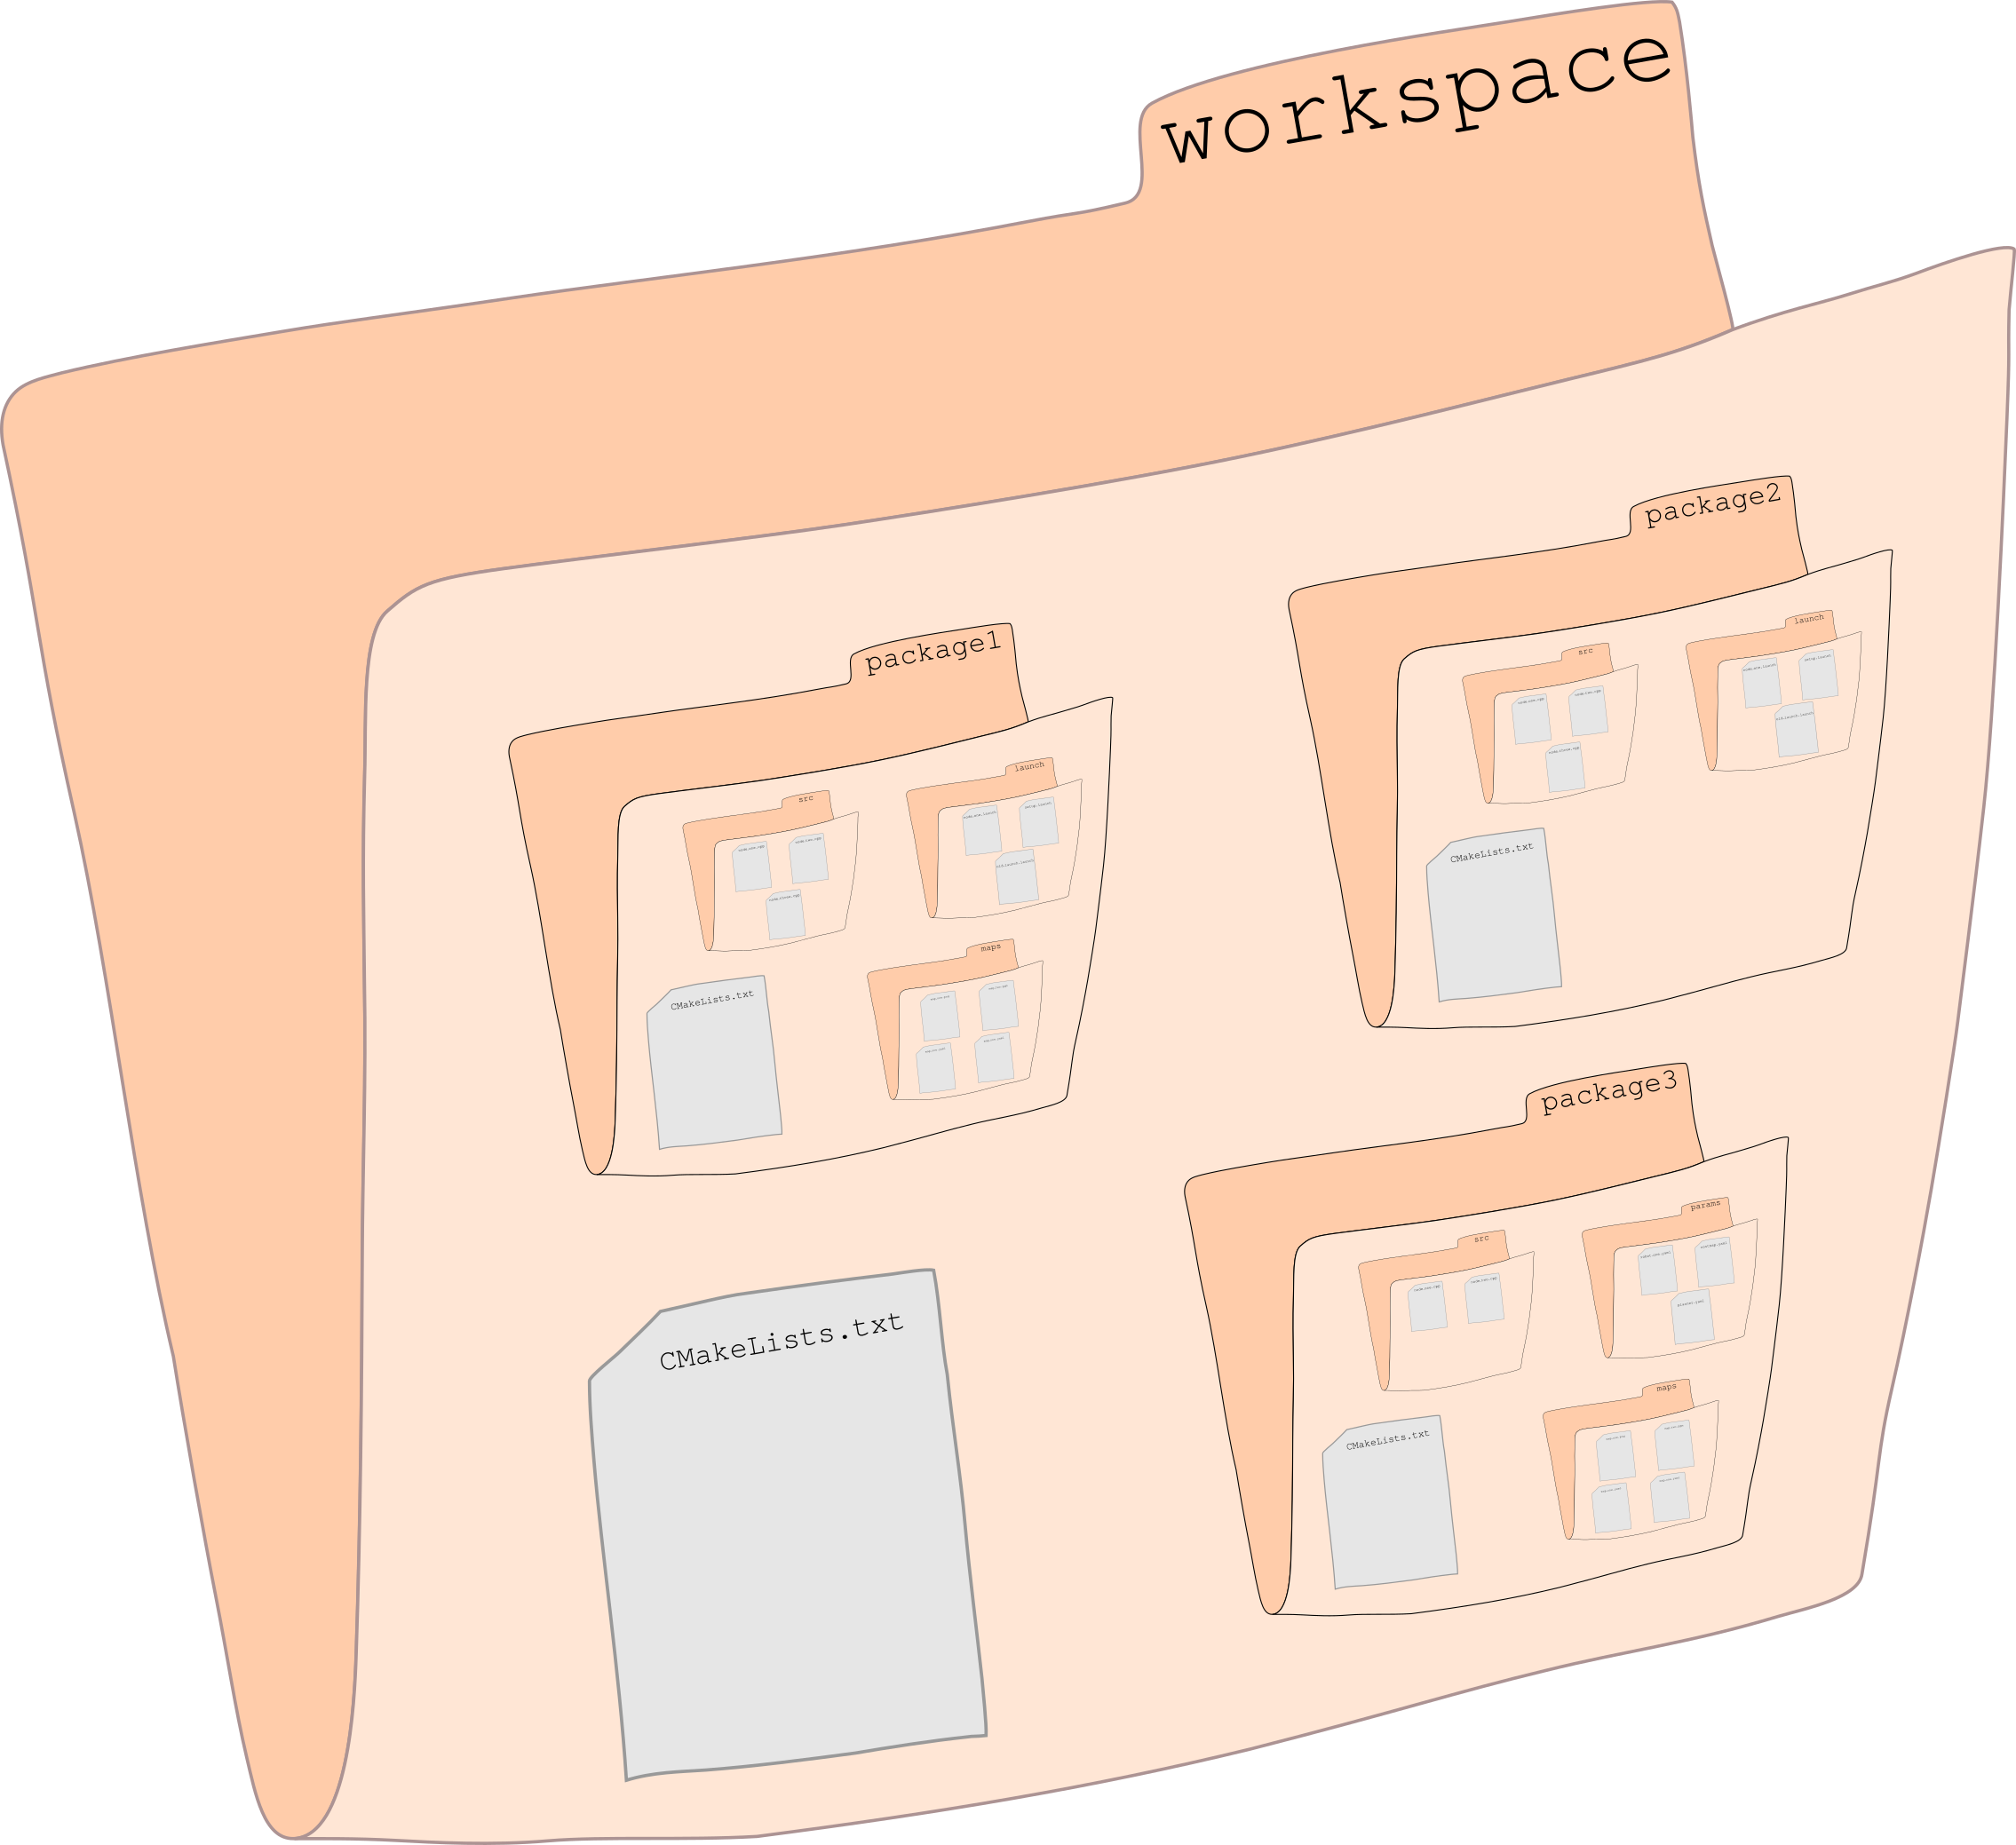
\includegraphics[scale=.15]{folders_small.png}
 

\end{frame}

\section{\sectiontitleIII}

	% Section II - Frame I
	\frame{ \small
		\frametitle{\sectiontitleIII}
		
		

}


\section{\sectiontitleIV}	
	% Section V - Frame I
	            \begin{frame}[label=sectionIV] \small
		\frametitle{\sectiontitleIV}    
	
 \setbeamertemplate{itemize items}[triangle]
                \begin{itemize}

					\item {\bf Overview:} You can customize your ROS system! Your exercise is to build a custom package and C++ node to control the turtlesim. 		

					\item {\bf Assignment:} Complete the tutorial in the document {\it tutorial4\_create\_package.pdf} on ilearn. Your custom package and node must  send a velocity command to the turtle and make it move without using the keyboard drive node.
                    
                    \item {\bf Deliverable:} Write a one to two paragraph summary of what you accomplished and what you struggled with the most. Include an image of the turtlesim window after your turtle has driven a pattern. 
    
                    \item {\bf Next Week:} After completion of Module 4, you are ready for a better robot. You will learn to use a simulated turtlebot3 in a Gazebo simulator. \vspc
                    
       
                \end{itemize}
		\end{frame}

\end{document}


